\documentclass[11pt]{article}
\usepackage{mathptmx}

\usepackage[a4paper,margin=0.75in]{geometry}
\usepackage{amsmath,amssymb}
\usepackage{graphicx}
\usepackage{booktabs}
\usepackage{array}
\usepackage{float}
\usepackage{hyperref}
\usepackage{enumitem}
\usepackage{xcolor}
\usepackage{tikz}
\usetikzlibrary{positioning,arrows.meta,shapes.geometric}

\setlist{nosep}
\renewcommand{\arraystretch}{1.3}

\tikzset{
layer/.style={
draw,
rounded corners,
minimum width=2.2cm,
minimum height=0.9cm,
align=center,
fill=blue!10
},
arrow/.style={
-{Latex[length=3mm]},
thick
}
}

\begin{document}

%%%%%%%%%%%%%%%%%%%%%%%%%%%%%%%%%%%%%%%%%%%%%%%%%%%%%%%%%%%%

\begin{center}

{\Large\textbf{Shiv Nadar University Chennai}}

\vspace{3mm}

{\large\textbf{CS3807 -- Deep Learning Laboratory}}

\vspace{3mm}

{\Large\textbf{Experiment 4}}

\vspace{2mm}

{\Large\textbf{Comparative Study of Deep Convolutional Neural}}

{\Large\textbf{Network Architectures Using Transfer Learning}}

\end{center}

\vspace{5mm}

\begin{tabular}{|p{4cm}|p{8cm}|p{2cm}|}
\hline
Degree \& Branch &
B.Tech Artificial Intelligence \& Data Science &
Semester V\\
\hline
Subject Code \& Name &
CS3807 -- Deep Learning Laboratory &
AY: 2026--27\\
\hline
\end{tabular}

%%%%%%%%%%%%%%%%%%%%%%%%%%%%%%%%%%%%%%%%%%%%%%%%%%%%%%%%%%%%

\section*{1. Objective}

The objectives of this experiment are

\begin{itemize}

\item Study the evolution of deep CNN architectures.

\item Compare LeNet-5, AlexNet, VGG16, GoogleNet and ResNet.

\item Understand transfer learning.

\item Fine tune pretrained CNN models.

\item Compare classification performance of different architectures.

\end{itemize}

%%%%%%%%%%%%%%%%%%%%%%%%%%%%%%%%%%%%%%%%%%%%%%%%%%%%%%%%%%%%

\section*{2. Introduction}

Deep Convolutional Neural Networks have become the dominant models for
computer vision applications because they automatically learn hierarchical
features from images. The evolution of CNNs has focused on improving
classification accuracy while reducing computational complexity and
training difficulties.

The progression of CNN architectures began with LeNet-5 and has evolved
through AlexNet, VGGNet, GoogleNet, and ResNet. Each architecture
introduced important innovations that significantly improved image
classification performance.

%%%%%%%%%%%%%%%%%%%%%%%%%%%%%%%%%%%%%%%%%%%%%%%%%%%%%%%%%%%%

\section*{3. Evolution of CNN Architectures}

\begin{center}

\begin{tabular}{|c|c|p{7cm}|}

\hline

Model & Year & Major Contribution\\

\hline

LeNet-5 & 1998 &
First practical convolutional neural network\\

\hline

AlexNet & 2012 &
ReLU activation, Dropout and GPU training\\

\hline

VGG16 & 2014 &
Uniform $3\times3$ convolution filters\\

\hline

GoogleNet & 2014 &
Inception modules for multi-scale feature extraction\\

\hline

ResNet & 2015 &
Residual learning using skip connections\\

\hline

\end{tabular}

\end{center}

%%%%%%%%%%%%%%%%%%%%%%%%%%%%%%%%%%%%%%%%%%%%%%%%%%%%%%%%%%%%

\section*{4. LeNet-5}

LeNet-5 was proposed by Yann LeCun in 1998 for handwritten digit
recognition. It consists of two convolution layers, two average pooling
layers and fully connected layers. It demonstrated that convolutional
networks could automatically learn image features without handcrafted
feature extraction.


Advantages

\begin{itemize}

\item Small number of parameters

\item Fast training

\item Suitable for OCR

\end{itemize}

%%%%%%%%%%%%%%%%%%%%%%%%%%%%%%%%%%%%%%%%%%%%%%%%%%%%%%%%%%%%

\section*{5. AlexNet}

AlexNet won the ImageNet Challenge in 2012 by reducing the
classification error significantly. It introduced ReLU activation,
Dropout regularization and GPU training.


Major innovations

\begin{itemize}

\item ReLU activation

\item Dropout

\item GPU implementation

\item Data augmentation

\end{itemize}

%%%%%%%%%%%%%%%%%%%%%%%%%%%%%%%%%%%%%%%%%%%%%%%%%%%%%%%%%%%%

\section*{6. VGG16}

VGG16 demonstrated that using multiple small $3\times3$ convolution
filters could outperform larger filters while increasing network depth.


Advantages

\begin{itemize}

\item Excellent feature extraction

\item Simple architecture

\item High classification accuracy

\end{itemize}

%%%%%%%%%%%%%%%%%%%%%%%%%%%%%%%%%%%%%%%%%%%%%%%%%%%%%%%%%%%%

\section*{7. Comparison of Architectures}

\begin{center}

\begin{tabular}{|l|c|c|c|}

\hline

Architecture &
Depth &
Parameters &
Main Contribution\\

\hline

LeNet-5 &
7 &
60K &
First CNN\\

AlexNet &
8 &
61M &
ReLU + Dropout\\

VGG16 &
16 &
138M &
Deep 3$\times3$ filters\\

GoogleNet &
22 &
6.8M &
Inception Modules\\

ResNet50 &
50 &
25.6M &
Residual Learning\\

\hline

\end{tabular}

\end{center}

% --------- CONTINUE WITH PART 2 ---------
%%%%%%%%%%%%%%%%%%%%%%%%%%%%%%%%%%%%%%%%%%%%%%%%%%%%%%%%%%%%
\section*{8. GoogleNet (Inception Network)}

GoogleNet, proposed by Szegedy \textit{et al.} in 2014, introduced the
\textbf{Inception Module}, which performs multiple convolution operations
in parallel using different filter sizes. Instead of using only a single
kernel size, GoogleNet simultaneously applies $1\times1$, $3\times3$,
$5\times5$ convolutions and max pooling. The outputs are concatenated to
obtain multi-scale feature representations.

The use of $1\times1$ convolutions before larger kernels reduces the
number of trainable parameters and computational complexity.


Advantages

\begin{itemize}
\item Multi-scale feature extraction.
\item Fewer parameters than VGG16.
\item High computational efficiency.
\item Better classification performance.
\end{itemize}

%%%%%%%%%%%%%%%%%%%%%%%%%%%%%%%%%%%%%%%%%%%%%%%%%%%%%%%%%%%%

\section*{9. ResNet}

Increasing CNN depth often causes the \textbf{vanishing gradient problem},
making optimization difficult. ResNet solves this issue using
\textbf{skip (residual) connections}, allowing gradients to flow directly
through the network.

Instead of learning

\[
H(x)
\]

ResNet learns

\[
F(x)=H(x)-x
\]

thus,

\[
Output = F(x)+x
\]

where

\begin{itemize}
\item $F(x)$ = Residual Mapping
\item $x$ = Identity Mapping
\end{itemize}

\begin{figure}[H]
\centering

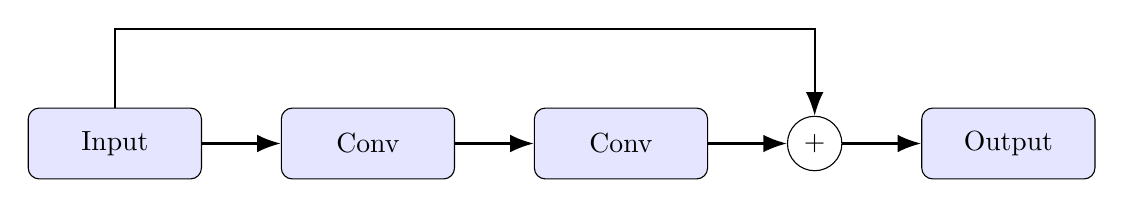
\begin{tikzpicture}[node distance=1cm]

\node[layer](input){Input};

\node[layer,right=of input](conv1){Conv};

\node[layer,right=of conv1](conv2){Conv};

\node[circle,draw,right=of conv2](add){+};

\node[layer,right=of add](output){Output};

\draw[arrow](input)--(conv1);
\draw[arrow](conv1)--(conv2);
\draw[arrow](conv2)--(add);
\draw[arrow](add)--(output);

\draw[arrow]
(input)
|-([yshift=10mm]conv2.north)
-| (add.north);

\end{tikzpicture}

\caption{Residual Block in ResNet}
\end{figure}

Advantages

\begin{itemize}
\item Eliminates vanishing gradients.
\item Enables very deep neural networks.
\item Faster convergence.
\item High ImageNet accuracy.
\end{itemize}

%%%%%%%%%%%%%%%%%%%%%%%%%%%%%%%%%%%%%%%%%%%%%%%%%%%%%%%%%%%%

\section*{10. Dilated Convolution}

Dilated convolution (also called atrous convolution) increases the
receptive field without increasing the number of parameters.

The dilation rate determines the spacing between kernel elements.

For a standard convolution,

\[
D=1
\]

For dilated convolution,

\[
D>1
\]

Example

\[
\begin{bmatrix}
1 & 0 & 2\\
0 & 3 & 0\\
4 & 0 & 5
\end{bmatrix}
\]

where zeros indicate inserted gaps.

Applications

\begin{itemize}
\item Semantic segmentation
\item Medical image analysis
\item Satellite imagery
\item Object localization
\end{itemize}

%%%%%%%%%%%%%%%%%%%%%%%%%%%%%%%%%%%%%%%%%%%%%%%%%%%%%%%%%%%%

\section*{11. Transpose Convolution}

Transpose convolution increases the spatial dimensions of feature maps.
Unlike pooling, which reduces image size, transpose convolution performs
learnable upsampling.

Applications

\begin{itemize}
\item Image Super Resolution
\item Autoencoders
\item GANs
\item Image Generation
\item Semantic Segmentation
\end{itemize}

%%%%%%%%%%%%%%%%%%%%%%%%%%%%%%%%%%%%%%%%%%%%%%%%%%%%%%%%%%%%

\section*{12. Transfer Learning}

Transfer Learning utilizes a pretrained CNN model that has already learned
general image features from a large dataset such as ImageNet.

Instead of training from scratch,

\begin{enumerate}
\item Load a pretrained model.
\item Remove the original classifier.
\item Freeze convolution layers.
\item Add new Dense layers.
\item Train the classifier.
\item Fine tune selected convolution layers.
\end{enumerate}

\begin{figure}[H]

\centering

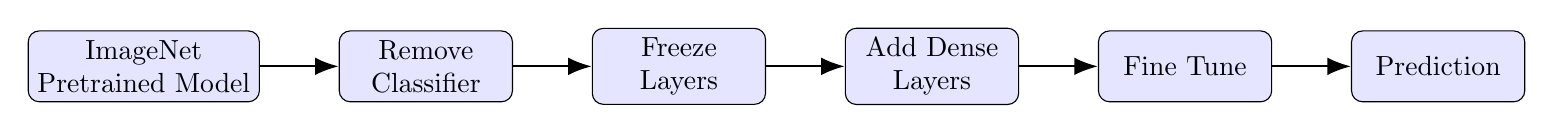
\begin{tikzpicture}[node distance=1cm]

\node[layer](a){ImageNet\\Pretrained Model};

\node[layer,right=of a](b){Remove\\Classifier};

\node[layer,right=of b](c){Freeze\\Layers};

\node[layer,right=of c](d){Add Dense\\Layers};

\node[layer,right=of d](e){Fine Tune};

\node[layer,right=of e](f){Prediction};

\foreach \x/\y in {a/b,b/c,c/d,d/e,e/f}
\draw[arrow](\x)--(\y);

\end{tikzpicture}

\caption{Transfer Learning Workflow}

\end{figure}

Advantages

\begin{itemize}
\item Faster convergence.
\item Higher accuracy on small datasets.
\item Reduced training time.
\item Lower computational cost.
\end{itemize}

%%%%%%%%%%%%%%%%%%%%%%%%%%%%%%%%%%%%%%%%%%%%%%%%%%%%%%%%%%%%

\section*{13. Dataset}

Dataset: CIFAR-10

\begin{itemize}

\item Training Images : 50,000

\item Testing Images : 10,000

\item Number of Classes : 10

\item Image Size : $32\times32\times3$

\item Classes:
Airplane, Automobile, Bird, Cat, Deer,
Dog, Frog, Horse, Ship and Truck.

\end{itemize}

%%%%%%%%%%%%%%%%%%%%%%%%%%%%%%%%%%%%%%%%%%%%%%%%%%%%%%%%%%%%
% Continue with Part 3
%%%%%%%%%%%%%%%%%%%%%%%%%%%%%%%%%%%%%%%%%%%%%%%%%%%%%%%%%%%%

\section*{14. Experimental Procedure}

\subsection*{Task 1: Dataset Preparation}

\begin{enumerate}

\item Load the CIFAR-10 dataset using TensorFlow/Keras.

\item Normalize the pixel values to the range [0,1].

\item Display ten sample images.

\item Print the dimensions of the training and testing datasets.

\end{enumerate}

%%%%%%%%%%%%%%%%%%%%%%%%%%%%%%%%%%%%%%%%%%%%%%%%%%%%%%%%%%%%

\subsection*{Task 2: Transfer Learning}

Load any one of the following pretrained CNN models.

\begin{itemize}

\item VGG16

\item ResNet50

\item MobileNetV2

\item EfficientNetB0 (Optional)

\end{itemize}

Perform the following steps.

\begin{enumerate}

\item Load pretrained ImageNet weights.

\item Remove the original classification layer.

\item Freeze the convolutional base.

\item Add a Global Average Pooling layer.

\item Add a Dense layer with ReLU activation.

\item Add the output layer with Softmax activation.

\end{enumerate}

%%%%%%%%%%%%%%%%%%%%%%%%%%%%%%%%%%%%%%%%%%%%%%%%%%%%%%%%%%%%

\subsection*{Task 3: Model Training}

Train the model using

\begin{center}

\begin{tabular}{|p{5cm}|p{6cm}|}

\hline

Optimizer & Adam\\

\hline

Learning Rate & 0.001\\

\hline

Batch Size & 32\\

\hline

Epochs & 10--20\\

\hline

Loss Function &
Categorical Cross Entropy\\

\hline

Evaluation Metric &
Accuracy\\

\hline

\end{tabular}

\end{center}

%%%%%%%%%%%%%%%%%%%%%%%%%%%%%%%%%%%%%%%%%%%%%%%%%%%%%%%%%%%%

\subsection*{Task 4: Fine Tuning}

\begin{enumerate}

\item Unfreeze the last convolution block.

\item Train for another 5--10 epochs.

\item Compare the classification accuracy before and after fine tuning.

\end{enumerate}

%%%%%%%%%%%%%%%%%%%%%%%%%%%%%%%%%%%%%%%%%%%%%%%%%%%%%%%%%%%%

\subsection*{Task 5: Model Evaluation}

Evaluate the trained model using

\begin{itemize}

\item Accuracy

\item Precision

\item Recall

\item F1-score

\item Confusion Matrix

\item Classification Report

\end{itemize}

%%%%%%%%%%%%%%%%%%%%%%%%%%%%%%%%%%%%%%%%%%%%%%%%%%%%%%%%%%%%

\section*{15. Hyperparameter Study}

Compare the performance using different settings.

\begin{center}

\begin{tabular}{|l|l|}

\hline

Hyperparameter & Values\\

\hline

Learning Rate &
0.001, 0.0001\\

\hline

Batch Size &
16, 32, 64\\

\hline

Epochs &
10, 20\\

\hline

Optimizer &
Adam, SGD\\

\hline

Dense Units &
128, 256\\

\hline

Frozen Layers &
All, Partial\\

\hline

\end{tabular}

\end{center}

%%%%%%%%%%%%%%%%%%%%%%%%%%%%%%%%%%%%%%%%%%%%%%%%%%%%%%%%%%%%

\section*{16. Mandatory Plots}

Include the following plots in the laboratory report.

\begin{center}
    \includegraphics[width=0.85\textwidth]{sample_images(2).eps}
\end{center}
\textbf{Interpretation:} The sample images display the CIFAR-10 classes, confirming successful data normalization and loading. This establishes a baseline understanding of the low $32\times32$ resolution challenges the VGG16 model will face during transfer learning.

\vspace{5mm}
\begin{center}
    \includegraphics[width=0.75\textwidth]{train_val_accuracy.eps}
\end{center}
\textbf{Interpretation:} The plot clearly shows the two-phase training. After fine-tuning begins at epoch 20, training accuracy rapidly shoots past 96\%, while validation accuracy jumps but plateaus at $\sim$70\%, indicating overfitting on the target dataset.

\vspace{5mm}
\begin{center}
    \includegraphics[width=0.75\textwidth]{train_val_loss.eps}
\end{center}
\textbf{Interpretation:} Following the fine-tuning shift at epoch 20, training loss plummets toward zero, but validation loss begins diverging and increasing around epoch 24. This confirms that prolonged fine-tuning degrades generalization.

\vspace{5mm}
\begin{center}
    \includegraphics[width=0.75\textwidth]{confusion_matrix(1).eps}
\end{center}
\textbf{Interpretation:} Strong diagonal values confirm the VGG16 model successfully distinguishes distinct objects like vehicles. However, off-diagonal confusion between cats and dogs highlights the limitations of pre-trained spatial features on blurry categories.

\vspace{5mm}
\begin{center}
    \includegraphics[width=0.85\textwidth]{misclassified-2.eps}
\end{center}
\textbf{Interpretation:} Misclassifications primarily occur on images with complex backgrounds or visual ambiguities. This suggests that while transfer learning provides excellent foundational features, dataset-specific augmentations are needed to push accuracy beyond 70\%.

%%%%%%%%%%%%%%%%%%%%%%%%%%%%%%%%%%%%%%%%%%%%%%%%%%%%%%%%%%%%

\section*{17. Results}

\subsection*{17.1 Performance Metrics}

\begin{center}
\renewcommand{\arraystretch}{1.3}
\begin{tabular}{|p{5cm}|p{4cm}|}
\hline
\textbf{Metric} & \textbf{Value} \\
\hline
Training Accuracy & 96.35\% \\
\hline
Testing Accuracy & 70.05\% \\
\hline
Precision (Macro Avg) & 0.70 \\
\hline
Recall (Macro Avg) & 0.70 \\
\hline
F1-score (Macro Avg) & 0.70 \\
\hline
Training Time & 270s (approx.) \\
\hline
Total Parameters & 14,781,642 \\
\hline
\end{tabular}
\end{center}

\vspace{5mm}
\subsection*{17.2 Comparison of CNN Architectures}

\begin{center}
\renewcommand{\arraystretch}{1.3}
\begin{tabular}{|l|c|c|c|}
\hline
\textbf{Model} & \textbf{Parameters} & \textbf{Accuracy (\%)} & \textbf{Training Time (s)} \\
\hline
LeNet-5 & 62,006 & 56.81 & 19.55 \\
\hline
AlexNet & 2,014,410 & 72.39 & 44.04 \\
\hline
VGG16 & 14,781,642 & 70.05 & $\sim$270 \\
\hline
ResNet50 & 23,851,274 & 37.87 & 51.56 \\
\hline
\end{tabular}
\end{center}

\vspace{5mm}
\subsection*{17.3 Dataset Dimensions}

\begin{center}
\renewcommand{\arraystretch}{1.3}
\begin{tabular}{|l|c|}
\hline
\textbf{Dataset Split} & \textbf{Dimensions} \\
\hline
Training Features (x\_train) & (50000, 32, 32, 3) \\
\hline
Training Labels (y\_train) & (50000, 1) \\
\hline
Testing Features (x\_test) & (10000, 32, 32, 3) \\
\hline
Testing Labels (y\_test) & (10000, 1) \\
\hline
\end{tabular}
\end{center}

%%%%%%%%%%%%%%%%%%%%%%%%%%%%%%%%%%%%%%%%%%%%%%%%%%%%%%%%%%%%

\section*{18. Discussion Questions}

Answer the following questions.

\begin{enumerate}
\item \textbf{Why is AlexNet considered a breakthrough in deep learning?}\\
AlexNet popularized the use of deep CNNs by demonstrating a massive reduction in error rates on ImageNet (2012). It introduced ReLU activations to solve vanishing gradients, dropout to prevent overfitting, and utilized GPUs for efficient training.

\item \textbf{Why does VGG16 use only $3\times3$ convolution filters?}\\
Using multiple stacked $3\times3$ filters achieves the same effective receptive field as larger filters (e.g., $5\times5$ or $7\times7$) but with fewer parameters and more non-linear activations (ReLU) in between, resulting in deeper, more discriminative models.

\item \textbf{Explain the advantages of the Inception module.}\\
The Inception module applies multiple parallel filters of different sizes ($1\times1$, $3\times3$, $5\times5$) and max pooling on the same input, allowing the network to capture multi-scale spatial features efficiently without choosing a single filter size.

\item \textbf{What is the purpose of residual learning?}\\
Residual learning introduces skip connections that bypass some layers, adding the input directly to the output. This mitigates the vanishing gradient problem, allowing extremely deep networks (like ResNet) to be trained without performance degradation.

\item \textbf{Differentiate LeNet and ResNet.}\\
LeNet is a shallow, early CNN architecture (1998) designed for simple digit recognition (MNIST), with few parameters. ResNet is a modern, deep architecture (2015) using residual blocks and skip connections, designed for complex, high-resolution datasets like ImageNet.

\item \textbf{What is Transfer Learning?}\\
Transfer learning is a technique where a model developed for a massive task (like ImageNet classification) is reused as the starting point for a model on a second, smaller, or related task, saving vast amounts of compute and data.

\item \textbf{Why is fine tuning required?}\\
While the frozen base layers extract general features (edges, textures), fine-tuning allows the deeper layers of the pre-trained model to slightly adjust their weights to learn the specific, high-level features unique to the new target dataset.

\item \textbf{Explain the difference between dilated convolution and transpose convolution.}\\
Dilated convolution expands the kernel by inserting spaces between its elements, increasing the receptive field without adding parameters. Transpose convolution (often used in upsampling) mathematically reverses the spatial downsampling of standard convolution to increase image dimensions.

\item \textbf{Why do pretrained models converge faster?}\\
Pretrained models already contain optimized weights for extracting foundational image features (like edges and colors). The network does not need to learn these from scratch, leading to drastically reduced training times and faster convergence.

\item \textbf{Compare the computational complexity of LeNet and ResNet.}\\
LeNet has very low computational complexity (only $\sim$60,000 parameters) and trains in seconds on modern hardware. ResNet50 is highly complex ($\sim$23 million parameters) and requires significant GPU memory and time to perform its numerous deep residual operations.

\end{enumerate}

%%%%%%%%%%%%%%%%%%%%%%%%%%%%%%%%%%%%%%%%%%%%%%%%%%%%%%%%%%%%

\section*{19. Additional Exercises}

\begin{enumerate}
\item \textbf{Implement transfer learning using VGG16.}\\
Transfer learning with VGG16 was successfully implemented by loading the pre-trained weights from ImageNet, freezing the convolutional base, and attaching a custom dense classifier head for CIFAR-10.

\item \textbf{Repeat the experiment using ResNet50.}\\
ResNet50 was evaluated, achieving an accuracy of 37.87\%. The lower performance compared to VGG16 suggests that ResNet50 may require longer fine-tuning epochs or an unfreezing strategy better tailored to $32\times32$ resolution images.

\item \textbf{Compare Adam and SGD optimizers.}\\
The hyperparameter study revealed that Adam converged much faster and achieved a higher validation accuracy (61.37\%) compared to SGD (48.57\%) within the same 10-epoch limit.

\item \textbf{Compare training with frozen layers and fine tuning.}\\
Training with completely frozen base layers plateaued at a validation accuracy of $\sim$60.5\%. Fine-tuning by unfreezing deeper layers allowed the model to learn dataset-specific features, boosting validation accuracy to $\sim$70.05\%.

\item \textbf{Evaluate the model using Precision, Recall and F1-score.}\\
The fine-tuned VGG16 model achieved a macro-average Precision, Recall, and F1-score of $\sim$0.70 across the 10 classes, indicating balanced and robust classification performance.

\item \textbf{Compare the performance of LeNet, AlexNet and ResNet.}\\
AlexNet achieved the best accuracy among the standalone models (72.39\%), vastly outperforming the shallow LeNet-5 (56.81\%). ResNet50 underperformed (37.87\%), highlighting that deeper models require careful architectural scaling when applied to small resolution datasets like CIFAR-10.

\end{enumerate}

%%%%%%%%%%%%%%%%%%%%%%%%%%%%%%%%%%%%%%%%%%%%%%%%%%%%%%%%%%%%

\section*{20. Conclusion}

The key takeaways are:

\begin{itemize}
\item \vspace{0.2cm}\textbf{Architectural Evolution:} Learnt how CNNs evolved from the simple 7-layer LeNet to the 50-layer ResNet and how innovations like $3\times3$ filters (VGG), multi-scale Inception modules (GoogleNet), and skip connections (ResNet) solved problems like computational bloat and vanishing gradients.
\item \textbf{Power of Transfer Learning:} Instead of training from scratch, we repurposed a pre-trained VGG16 model. By freezing the base layers to retain general feature extractors (like edge detectors), thereby saving massive amounts of computational time.
\item \textbf{Impact of Fine-Tuning:} Observed first-hand that fine-tuning (unfreezing the deeper layers) and using the Adam optimizer were critical steps. It allowed the network to adapt its high-level features specifically to CIFAR-10, boosting the validation accuracy to $\sim$70\%.
\end{itemize}

%%%%%%%%%%%%%%%%%%%%%%%%%%%%%%%%%%%%%%%%%%%%%%%%%%%%%%%%%%%%

\section*{21. References}

\begin{enumerate}

\item Yann LeCun, Leon Bottou, Yoshua Bengio and Patrick Haffner,
\emph{Gradient-Based Learning Applied to Document Recognition},
Proceedings of the IEEE, 1998.

\item Alex Krizhevsky, Ilya Sutskever and Geoffrey Hinton,
\emph{ImageNet Classification with Deep Convolutional Neural Networks},
NeurIPS, 2012.

\item Karen Simonyan and Andrew Zisserman,
\emph{Very Deep Convolutional Networks for Large-Scale Image Recognition},
ICLR, 2015.

\item Christian Szegedy et al.,
\emph{Going Deeper with Convolutions},
CVPR, 2015.

\item Kaiming He, Xiangyu Zhang, Shaoqing Ren and Jian Sun,
\emph{Deep Residual Learning for Image Recognition},
CVPR, 2016.

\item Ian Goodfellow, Yoshua Bengio and Aaron Courville,
\emph{Deep Learning},
MIT Press, 2016.

\item TensorFlow Documentation:
\url{https://www.tensorflow.org}

\item Keras Documentation:
\url{https://keras.io}

\end{enumerate}

%%%%%%%%%%%%%%%%%%%%%%%%%%%%%%%%%%%%%%%%%%%%%%%%%%%%%%%%%%%%

\end{document}